%%%%%%%%%%%%%%%%%%%%%%%%%%%%%%%%%%%%%%%%%
% Beamer Presentation
% LaTeX Template
% Version 1.0 (10/11/12)
%
% This template has been downloaded from:
% http://www.LaTeXTemplates.com
%
% License:
% CC BY-NC-SA 3.0 (http://creativecommons.org/licenses/by-nc-sa/3.0/)
%
%%%%%%%%%%%%%%%%%%%%%%%%%%%%%%%%%%%%%%%%%

%----------------------------------------------------------------------------------------
%	PACKAGES AND THEMES
%----------------------------------------------------------------------------------------

%\documentclass[UTF8,aspectratio=169,14pt]{ctexbeamer}
\documentclass[UTF8,aspectratio=169]{ctexbeamer}
\usepackage{hyperref}
\hypersetup{
	colorlinks=true,
	linkcolor=red,
	anchorcolor=blue,
	citecolor=green
}

\mode<presentation> {
	
	% The Beamer class comes with a number of default slide themes
	% which change the colors and layouts of slides. Below this is a list
	% of all the themes, uncomment each in turn to see what they look like.
	
	%\usetheme{default}
	%\usetheme{AnnArbor}
	%\usetheme{Antibes}
	%\usetheme{Bergen}
	%\usetheme{Berkeley}
	%\usetheme{Berlin}
	%\usetheme{Boadilla}
	%\usetheme{CambridgeUS}
	%\usetheme{Copenhagen}
	%\usetheme{Darmstadt}
	%\usetheme{Dresden}
	%\usetheme{Frankfurt}
	%\usetheme{Goettingen}
	%\usetheme{Hannover}
	%\usetheme{Ilmenau}
	%\usetheme{JuanLesPins}
	%\usetheme{Luebeck}
	\usetheme{Madrid}
	%\usetheme{Malmoe}
	%\usetheme{Marburg}
	%\usetheme{Montpellier}
	%\usetheme{PaloAlto}
	%\usetheme{Pittsburgh}
	%\usetheme{Rochester}
	%\usetheme{Singapore}
	%\usetheme{Szeged}
	%\usetheme{Warsaw}
	
	% As well as themes, the Beamer class has a number of color themes
	% for any slide theme. Uncomment each of these in turn to see how it
	% changes the colors of your current slide theme.
	
	%\usecolortheme{albatross}
	%\usecolortheme{beaver}
	%\usecolortheme{beetle}
	%\usecolortheme{crane}
	%\usecolortheme{dolphin}
	%\usecolortheme{dove}
	%\usecolortheme{fly}
	%\usecolortheme{lily}
	%\usecolortheme{orchid}
	%\usecolortheme{rose}
	%\usecolortheme{seagull}
	%\usecolortheme{seahorse}
	%\usecolortheme{whale}
	%\usecolortheme{wolverine}
	
	%\setbeamertemplate{footline} % To remove the footer line in all slides uncomment this line
	%\setbeamertemplate{footline}[page number] % To replace the footer line in all slides with a simple slide count uncomment this line
	
	%\setbeamertemplate{navigation symbols}{} % To remove the navigation symbols from the bottom of all slides uncomment this line
}

\usepackage{graphicx} % Allows including images
\graphicspath{{./figs/}}
\usepackage{booktabs} % Allows the use of \toprule, \midrule and \bottomrule in tables
\usepackage{longtable}
\usepackage{listings}
\usepackage{xcolor}
\lstset{numbers=left, %设置行号位置
	numberstyle=\tiny, %设置行号大小
	keywordstyle=\color{blue}, %设置关键字颜色
	commentstyle=\color[cmyk]{1,0,1,0}, %设置注释颜色
	frame=single, %设置边框格式
	escapeinside=``, %逃逸字符(1左面的键),用于显示中文
	%breaklines, %自动折行
	extendedchars=false, %解决代码跨页时,章节标题,页眉等汉字不显示的问题
	xleftmargin=2em,xrightmargin=2em, aboveskip=1em, %设置边距
	tabsize=4, %设置tab空格数
	showspaces=false %不显示空格
}
% Fonts
% \usepackage{libertine}
% \setmonofont{Courier}
\setCJKsansfont[ItalicFont=Noto Serif CJK SC Black, BoldFont=Noto Sans CJK SC Black]{Noto Sans CJK SC}
\setmainfont[Ligatures={Common,TeX}]{Linux  Libertine O}
\setmonofont[SmallCapsFont={Latin Modern Mono Caps}]{Latin Modern Mono Light}
\setsansfont{Linux Biolinum O}

\logo{
\includegraphics[width=0.55cm,height=0.55cm]{../../thcs-logo.png}}

%----------------------------------------------------------------------------------------
%	TITLE PAGE
%----------------------------------------------------------------------------------------

\title[第4讲]{第4讲 :Optimization of Virtual Machine Monitor} % The short title appears at the bottom of every slide, the full title is only on the title page
\subtitle{第三节:Dune: Safe User-level Access to Privileged CPU Features}
\author{陈渝} % Your name
\institute[清华大学] % Your institution as it will appear on the bottom of every slide, may be shorthand to save space
{
	清华大学计算机系 \\ % Your institution for the title page
	\medskip
	\textit{yuchen@tsinghua.edu.cn} % Your email address
}
\date{\today} % Date, can be changed to a custom date


\begin{document}

\begin{frame}
\titlepage % Print the title page as the first slide
\end{frame}

%\begin{frame}
%\frametitle{提纲} % Table of contents slide, comment this block out to remove it
%\tableofcontents % Throughout your presentation, if you choose to use \section{} and \subsection{} commands, these will automatically be printed on this slide as an overview of your presentation
%\end{frame}
%
%%----------------------------------------------------------------------------------------
%%	PRESENTATION SLIDES
%%----------------------------------------------------------------------------------------
%
%%------------------------------------------------
%\section{第一节:课程概述} % Sections can be created in order to organize your presentation into discrete blocks, all sections and subsections are automatically printed in the table of contents as an overview of the talk
%%------------------------------------------------


%-------------------------------------------------
\begin{frame}[plain]
	\frametitle{Requirement of DUNE}
	
	
	
	\begin{columns}
		
		\begin{column}{.4\textwidth}
			
			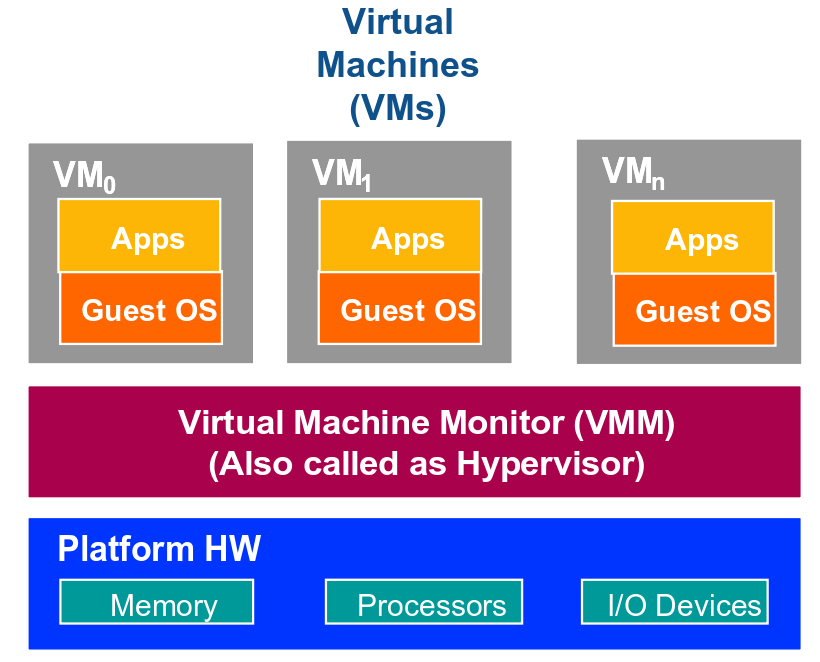
\includegraphics[width=1.\textwidth]{vmm-overview}
			
		\end{column}
		
		\begin{column}{.7\textwidth}
			
			\LARGE
			\underline{\textbf{For MORE performance \& features}}
			
			\large
			Safe	
 User -‐ level	
 Access	
 to Privileged	
 CPU	
 Features			
			
		\end{column}
		
		
	\end{columns}
	\tiny Dune:	
 Safe	
 User-­‐level	
 Access
 to 	Privileged	
 CPU	
 Features, Adam 
 Belay,etc.,	OSDI'12

\end{frame}


%-------------------------------------------------
\begin{frame}[plain]
	\frametitle{Requirement of DUNE}
	
	
	
	\begin{columns}
		
		\begin{column}{.4\textwidth}
			
			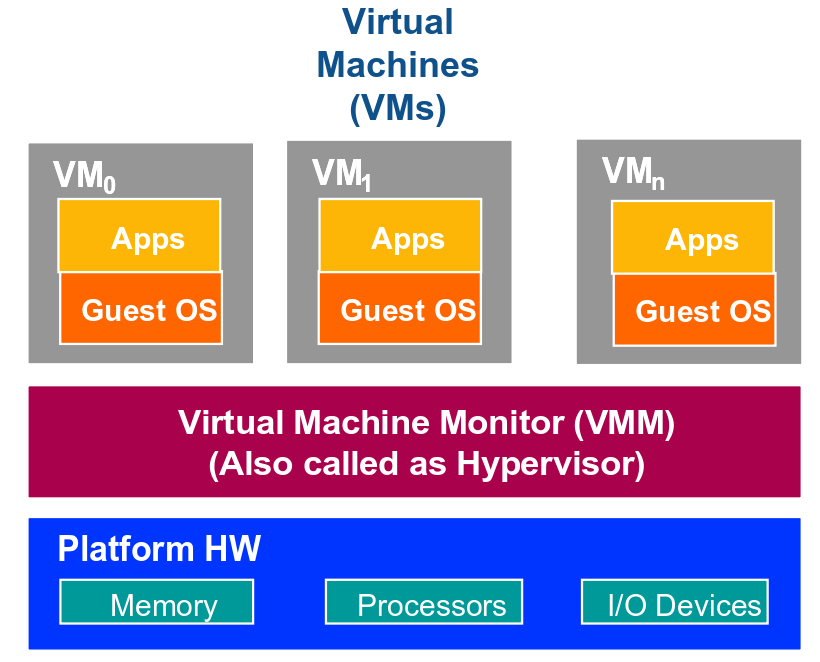
\includegraphics[width=1.\textwidth]{vmm-overview}
			
		\end{column}
		
		\begin{column}{.6\textwidth}
			
			\Large
			\underline{\textbf{For MORE performance \& features}}
		\small	
		\begin{itemize}
	\item Speed	 up	 garbage	 collection	 (Azul	 C4)	
	
	pagetable
    \item Privilege separaAon	 within	 a	 process	 (Palladium)
    
    MMU	
	\item Safe	 native code	 in	 web	 browsers	 (Xax) 
	
	Syscall handler
	
\end{itemize}		
			
		\end{column}
		
		
	\end{columns}

	
\end{frame}



%-------------------------------------------------
\begin{frame}[plain]
	\frametitle{ Some thoughts of DUNE -- Change kernel}
	
			\centering
			\Large
			Problem:	
 stability	
 concerns,	
 challenging	
 to	
  OpAmizaAon	
 analysis
			distribute,	
 composability	
 concerns	
  
			
			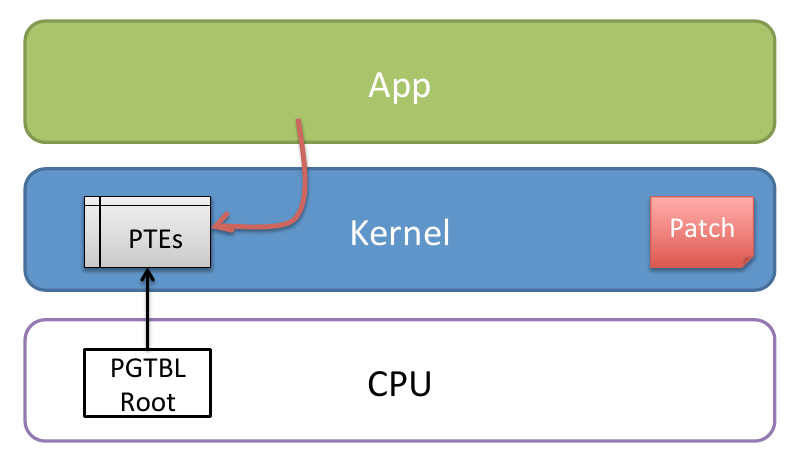
\includegraphics[width=.7\textwidth]{change-kernel}
			
	
	
\end{frame}


%-------------------------------------------------
\begin{frame}[plain]
	\frametitle{ Some thoughts of DUNE -- exokernel}
	
	\centering
	\Large
	Problem:	 must	 replace	 entire	 OS	 stack	
  
	
	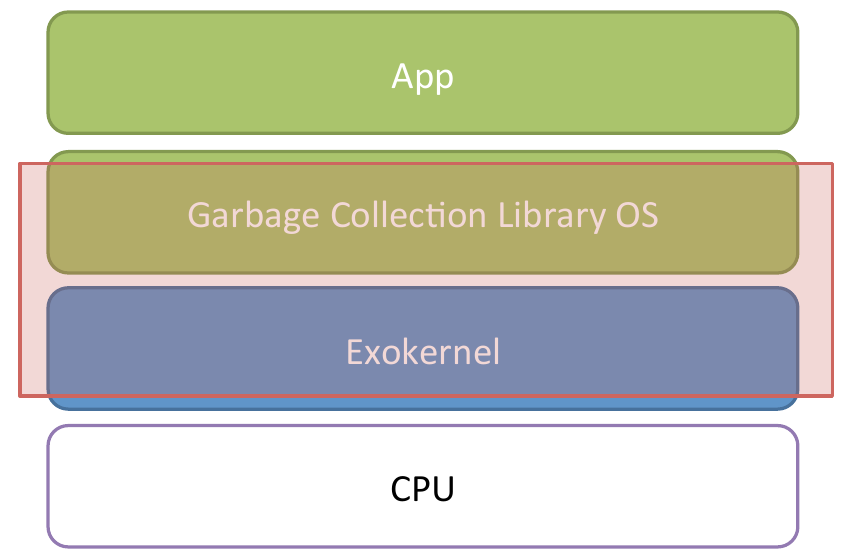
\includegraphics[width=.7\textwidth]{change-exokernel}
	
	
	
\end{frame}


%-------------------------------------------------
\begin{frame}[plain]
	\frametitle{ Some thoughts of DUNE -- VMM}
	
	\centering
	\Large
	Problem:	virtual	machines	have	strict	partitioning	
  
	
	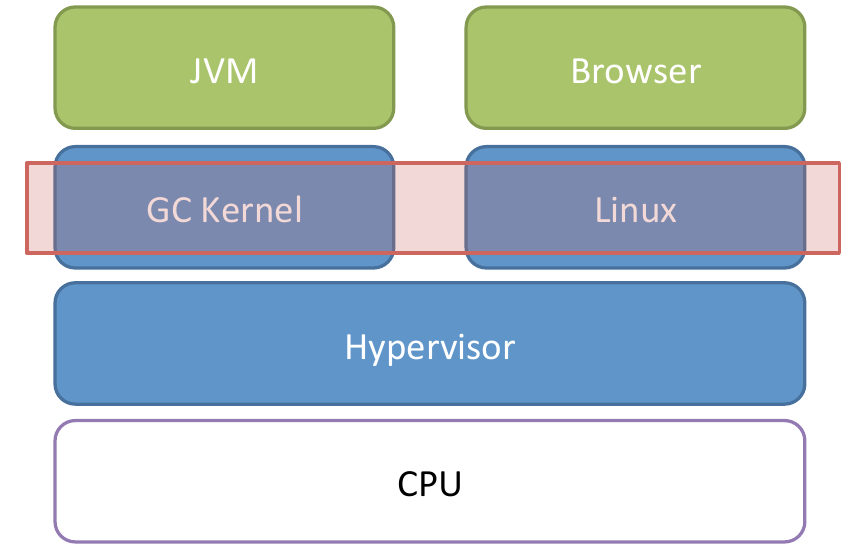
\includegraphics[width=.7\textwidth]{change-vmm}
	
	
	
\end{frame}


%-------------------------------------------------
\begin{frame}[plain]
	\frametitle{ Some thoughts of DUNE -- Dune in a Nutshell}
	
	\centering
	
  
	
	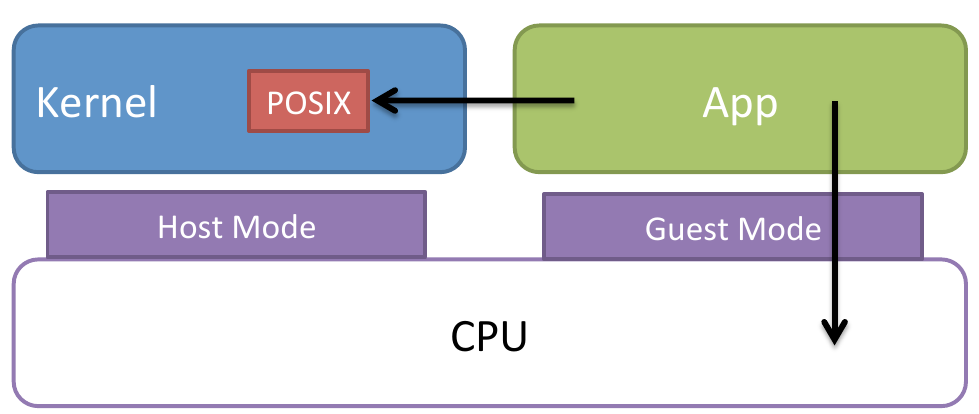
\includegraphics[width=.7\textwidth]{dune-nutshell}
	\centering
	\begin{itemize}
		\item Provide	 safe user-­‐level	 access	 to	 privileged	 CPU	 features
		\item Still  a	 normal	 process	 in	 all	 ways	 (POSIX	 API,	 etc)	
		\item Key
 idea:
 leverage existing virtualization hardware (VT‐x)	
  		
	\end{itemize}		
	
\end{frame}


%-------------------------------------------------
\begin{frame}[plain]
	\frametitle{ Some thoughts of DUNE -- Dune Simple Arch}
	
	\centering
	
	
	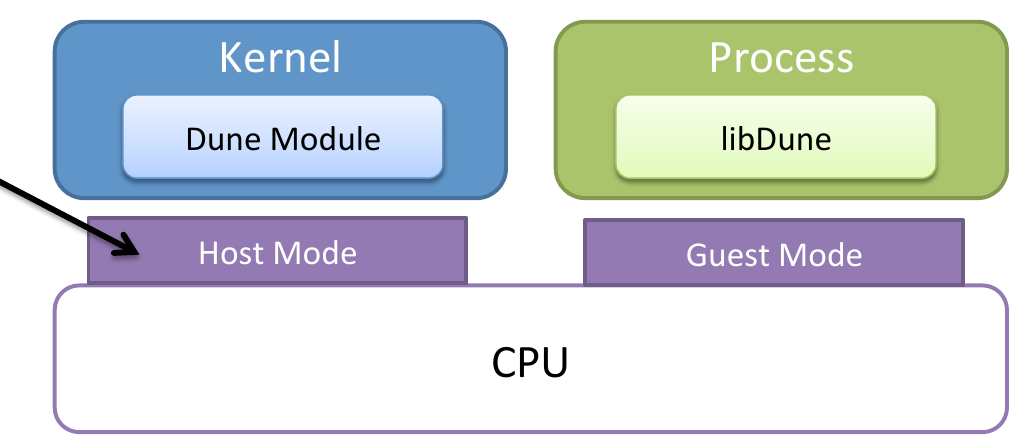
\includegraphics[width=.7\textwidth]{dune-simple-arch}
	\centering
	\begin{itemize}
		\item Host	
 mode	
 -­‐>	
 VMX	
 root	
 mode	
 on	
 Intel	
  
		
		\item Normally	 used	 for	 hypervisors	

		\item In Dune,	we	run	the	kernel	here,for access VT-x instructions.	 		
	\end{itemize}		
	
\end{frame}


%-------------------------------------------------
\begin{frame}[plain]
	\frametitle{ Some thoughts of DUNE -- Dune Simple Arch}
	
	\centering
	
	
	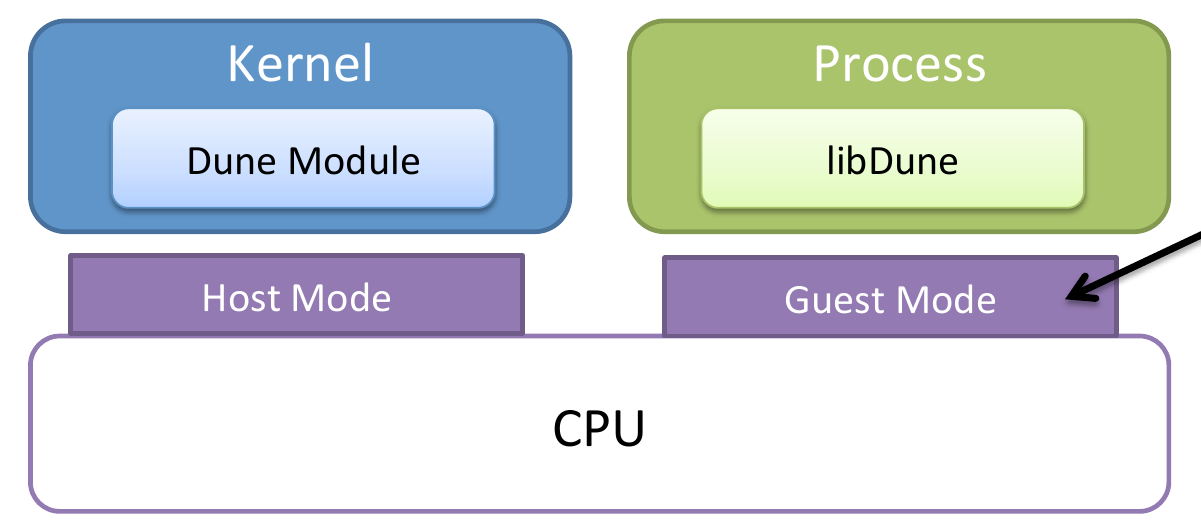
\includegraphics[width=.7\textwidth]{dune-simple-arch-guest}
	\centering
	\begin{itemize}
		\item Guest	
 mode	
 -­‐>	
 VMX	
 non-­‐root	
 mode	
 on	
 Intel	
  
			
  
		
		\item Normally	 used by	 the	 guest	 kernel	
		
		\item In Dune, we	
 run	
 ordinary	
 processes	
 here, for access	
 to	
 privileged	
 features		
	\end{itemize}		
	
\end{frame}


%-------------------------------------------------
\begin{frame}[plain]
	\frametitle{ Some thoughts of DUNE -- Dune Simple Arch}
	
	\centering
	
	
	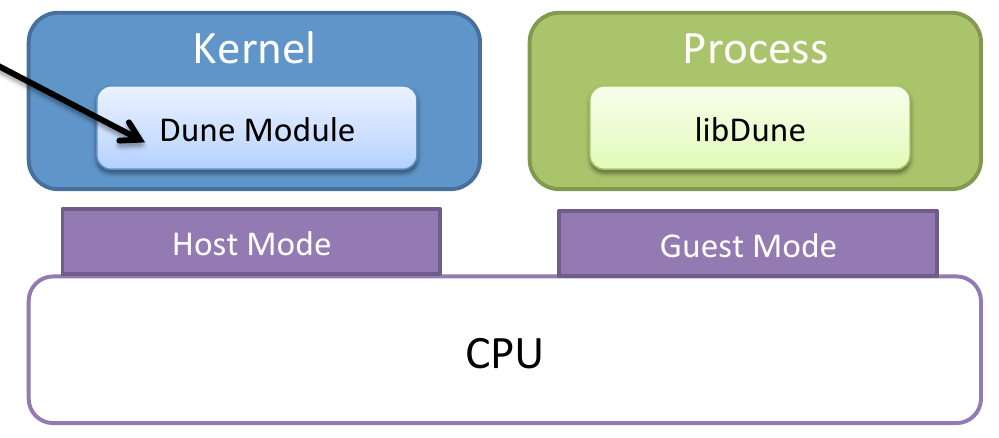
\includegraphics[width=.7\textwidth]{dune-simple-arch-module}
	\centering
	\begin{itemize}
		\item Configures	 and manages	 virtualization	 hardware		
  		
		
		\item Provides	
 integration	
 with	
 the	
 rest	
 of	
 the	
 kernel	
 in	
 order	
 to	
 support	
 a	
  		process	
 abstraction
		
		\item Uses	 Intel VT‐x		
	\end{itemize}		
	
\end{frame}


%-------------------------------------------------
\begin{frame}[plain]
	\frametitle{ Some thoughts of DUNE -- Dune Simple Arch}
	
	\centering
	
	
	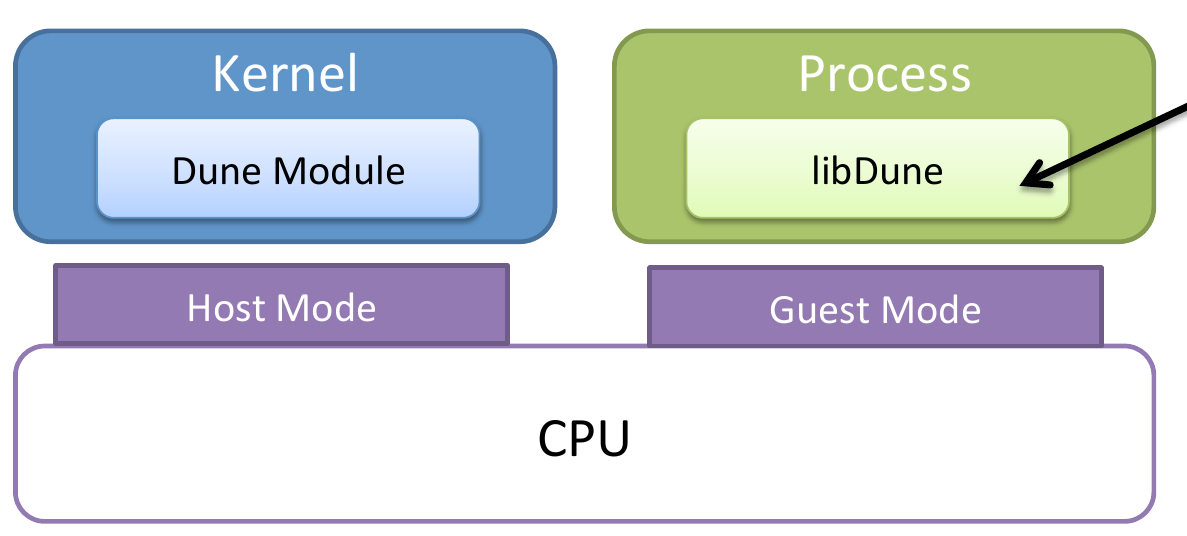
\includegraphics[width=.7\textwidth]{dune-simple-arch-lib}
	\centering
	\begin{itemize}
		\item A	
 uAlity	
 library	
 to	
 help	
 applicaAons	
 manage	
 privileged	
 hardware	
  		features		
  		
		
		\item Completely	 untrusted
		
		\item Exception	
 handling,	
 syscall	
 handling,	
 page	
 allocator,	
 page	
 table	
  		management,	
 ELF	
 loader	
 
	\end{itemize}		
	
\end{frame}
%-------------------------------------------------
\begin{frame}[plain]
	\frametitle{Diff Between VMM \& DUNE}
	
	
	
	\begin{columns}
		
		\begin{column}{.5\textwidth}
			
			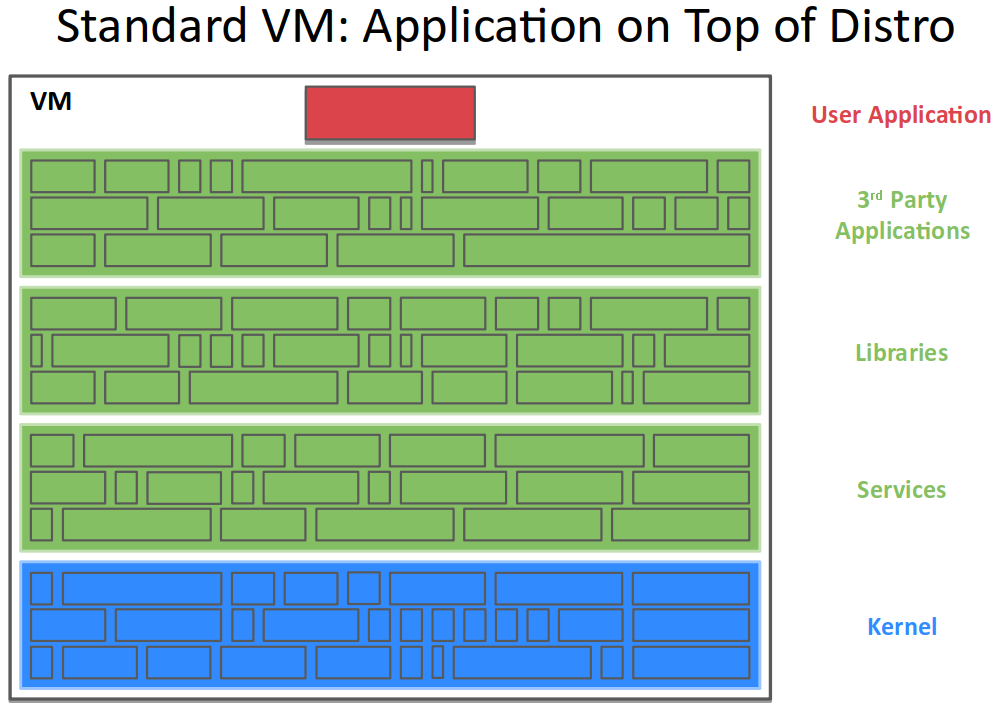
\includegraphics[width=1.\textwidth]{standard-vm}
			
		\end{column}
		
		\begin{column}{.5\textwidth}
			\centering
			DUNE:  using virtualization hardware to provide a process
			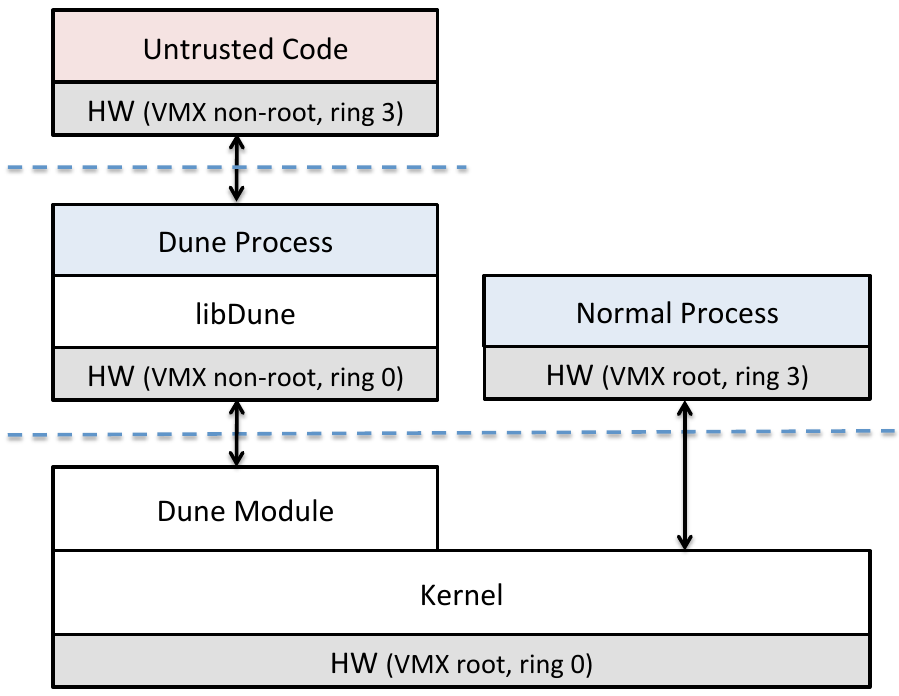
\includegraphics[width=1.\textwidth]{dune-arch}			
			
		\end{column}
		
		
	\end{columns}
	
	
\end{frame}


%-------------------------------------------------
\begin{frame}[plain]
	\frametitle{Contributions of DUNE}
	
	
	
	\begin{columns}
		
		\begin{column}{.4\textwidth}
			\centering
			DUNE
			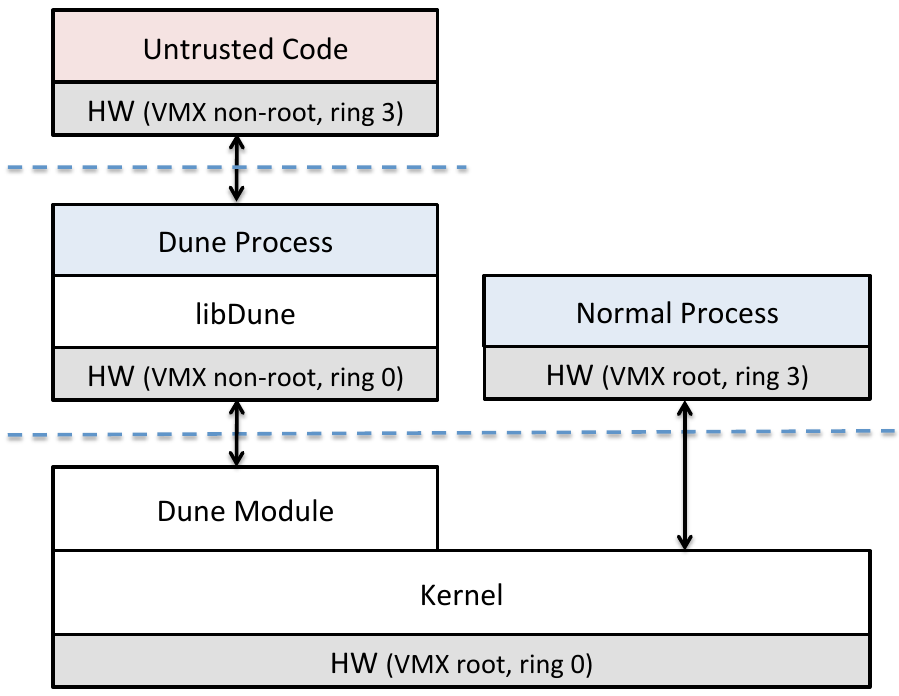
\includegraphics[width=1.\textwidth]{dune-arch}
			
		\end{column}
		
		\begin{column}{.6\textwidth}

		\begin{itemize}
			\item a design that uses hardware-assisted virtualization to safely and efficiently expose privileged hardware features to user programs while preserving standard OS abstractions.
			\Large
			\begin{itemize}
				\item Memory	 management	
				\item System	 calls
 				\item POSIX	 Signals	
			\end{itemize}
%			\item evaluate three hardware features in detail and show
%			how they can benefit user programs: exceptions, paging, and privilege modes.
%			\item demonstrate the end-to-end utility of Dune by implementing and evaluating three use cases: sandboxing,
%			privilege separation, and garbage collection.
			
		\end{itemize}						
			
		\end{column}
		
		
	\end{columns}
	
	
\end{frame}


%-------------------------------------------------
\begin{frame}[plain]
	\frametitle{Supported Hardware Features}
	
	
	
	\begin{columns}
		
		\begin{column}{.4\textwidth}
	
			
			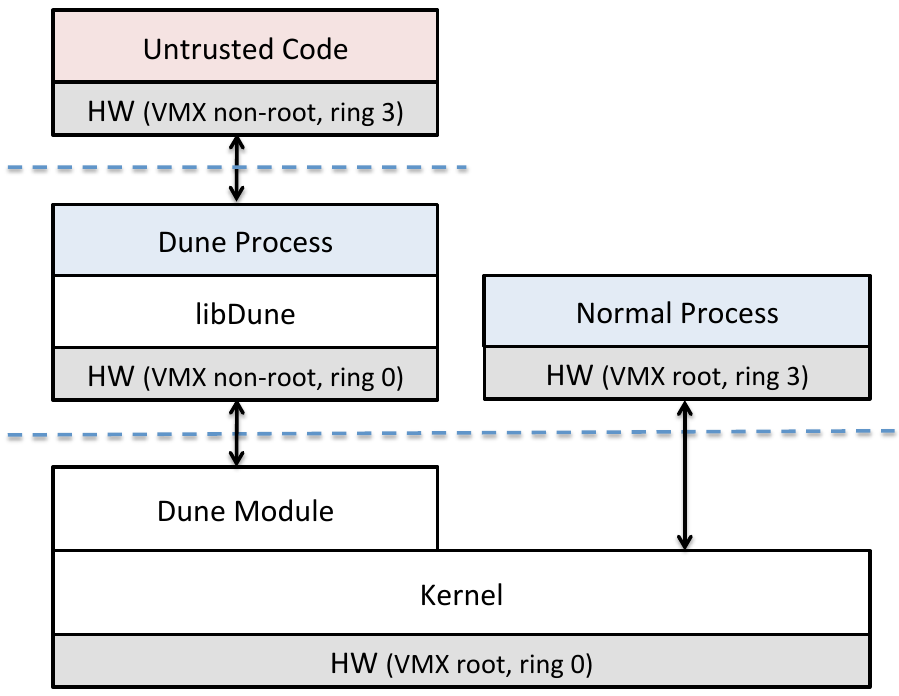
\includegraphics[width=1.\textwidth]{dune-arch}
			
		\end{column}
		
		\begin{column}{.6\textwidth}
			\centering
			Hardware features exposed by Dune and their corresponding privileged x86 instructions.

			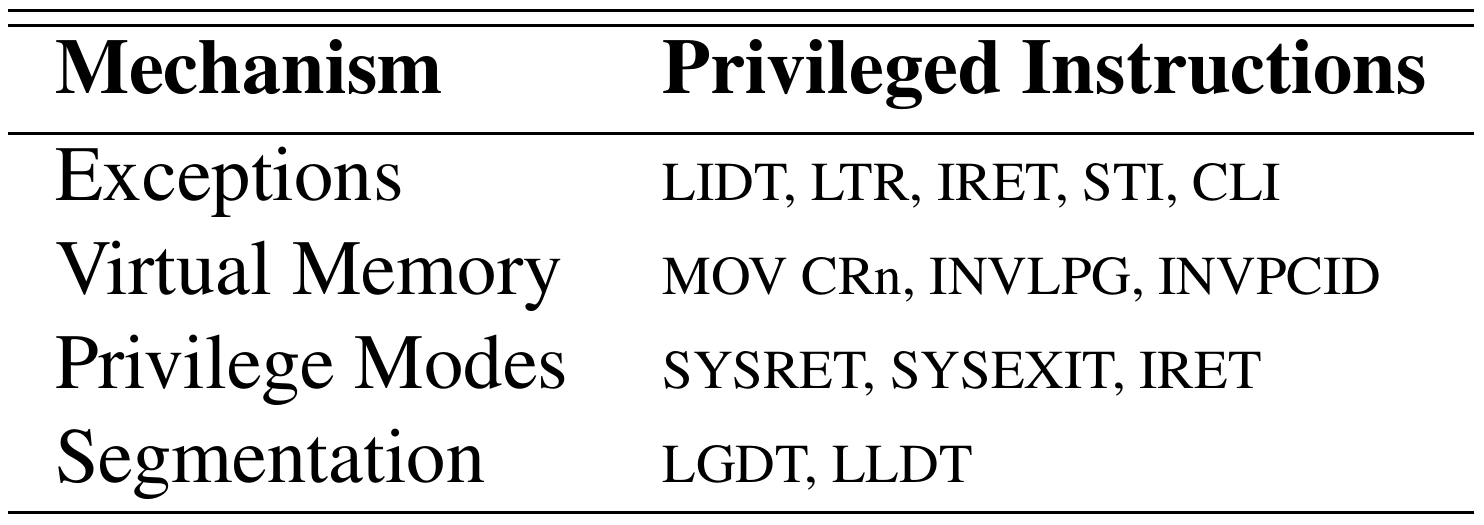
\includegraphics[width=.9\textwidth]{hw-features}					
			
		\end{column}
		
		
	\end{columns}
	
	
\end{frame}


%-------------------------------------------------
\begin{frame}[plain]
	\frametitle{Supported Hardware Features -- Exceptions}
	
	
	
	\begin{columns}
		
		\begin{column}{.4\textwidth}
			\centering
			Hardware features exposed by Dune
			
			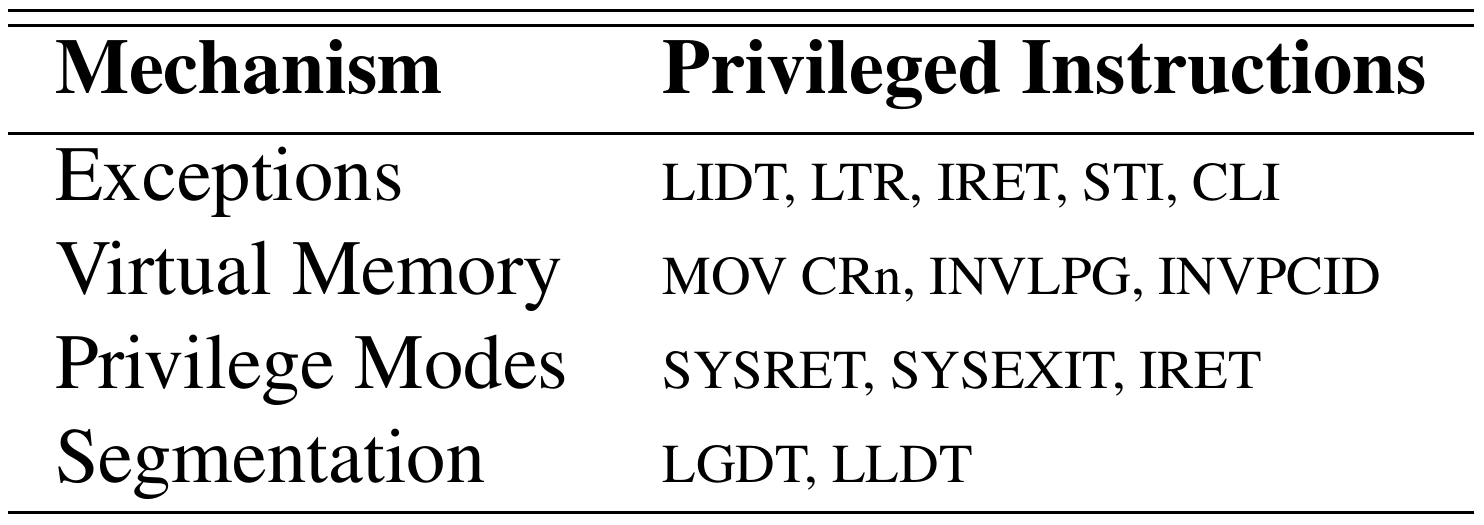
\includegraphics[width=1.\textwidth]{hw-features}
			
		\end{column}
		
		\begin{column}{.6\textwidth}


		\begin{itemize}
	\item Normally, reporting an exception to a
	user program requires privilege mode transitions and an
	upcall mechanism (e.g., signals)
	\item Dune can reduce exception overhead because it uses VT-x to deliver exceptions directly in hardware.
	\item proves the speed of delivering page fault exceptions by more than 4 X
		\end{itemize}					
			
		\end{column}
		
		
	\end{columns}
	
	
\end{frame}


%-------------------------------------------------
\begin{frame}[plain]
	\frametitle{Supported Hardware Features -- Virtual Memory}
	
	
	
	\begin{columns}
		
		\begin{column}{.4\textwidth}
			\centering
			Hardware features exposed by Dune
			
			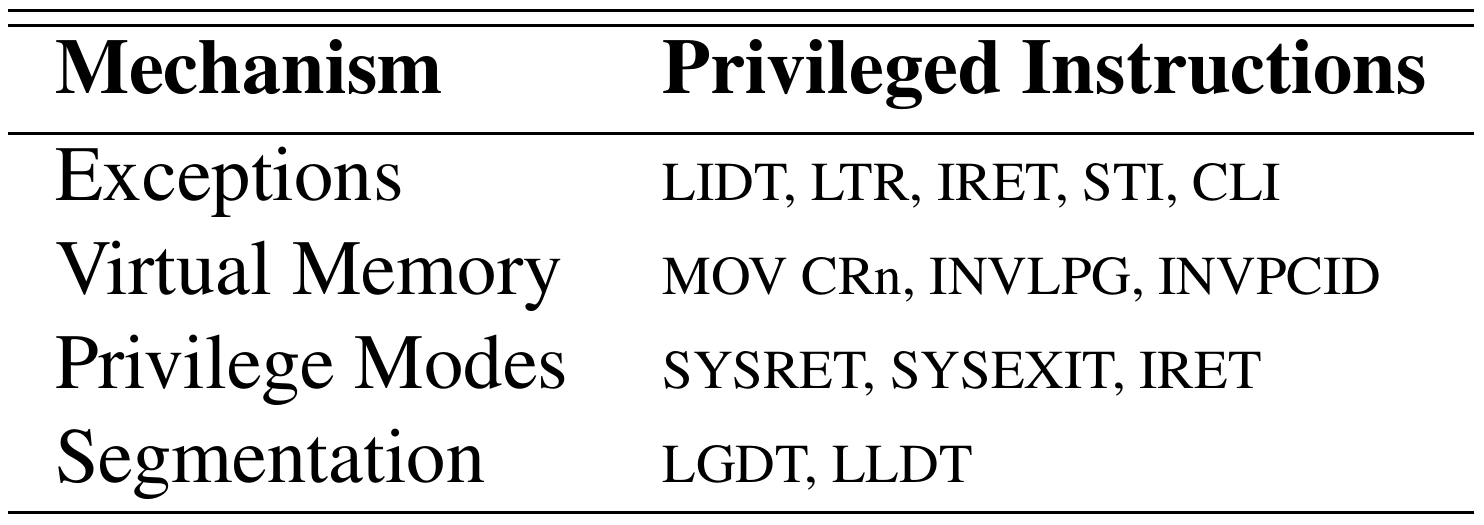
\includegraphics[width=1.\textwidth]{hw-features}
			
		\end{column}
		
		\begin{column}{.6\textwidth}
			
			
			\begin{itemize}
				\item  gives user programs the ability to manually
				control TLB invalidations.
				\item page table updates
				can be performed in batches when permitted by the application. 
				\item Dune exposes TLB tagging by providing access to Intel’s recently added process-context identifier (PCID) feature
				\item Dune results in a 7× speedup		over Linux in the Appel and Li user-level virtual memory		benchmarks 
				
			\end{itemize}					
			
		\end{column}
		Uses	 Intel VT‐x		
		
	\end{columns}
	
	
\end{frame}



%-------------------------------------------------
\begin{frame}[plain]
	\frametitle{ Supported Hardware Features -- Virtual Memory}
	
	\centering
	
	
	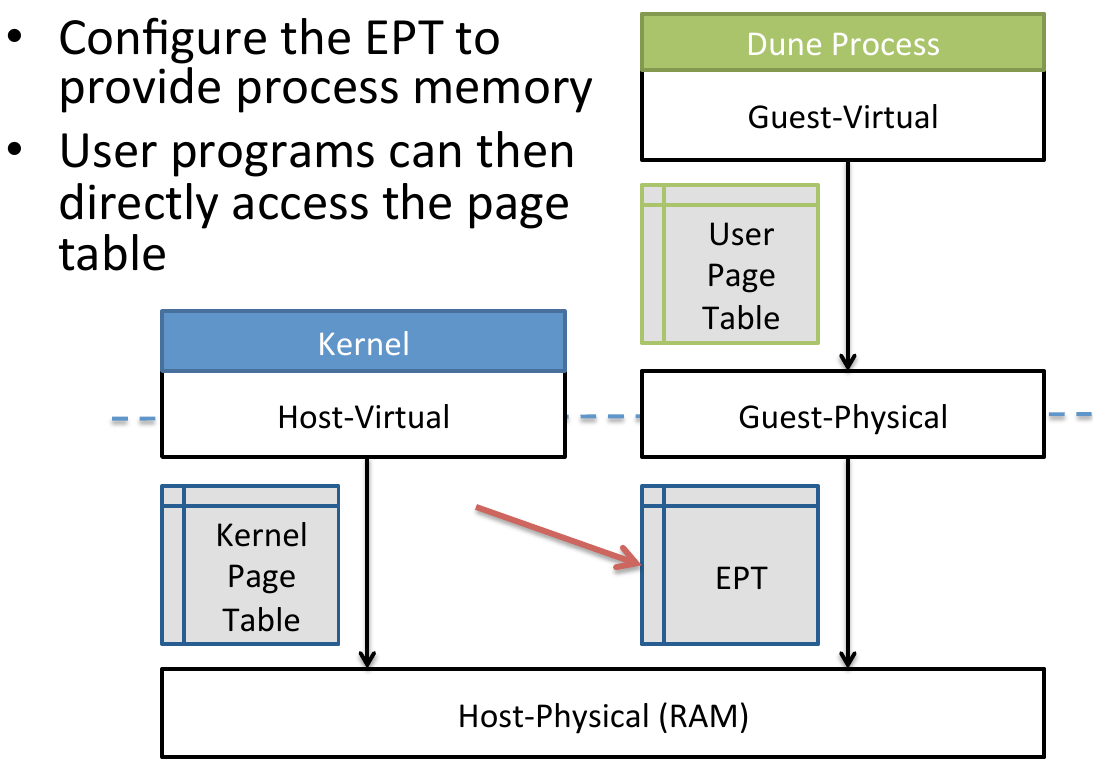
\includegraphics[width=.7\textwidth]{dune-hw-virtmem}

	
\end{frame}
%-------------------------------------------------
\begin{frame}[plain]
	\frametitle{Supported Hardware Features -- Privilege Modes}
	
	
	
	\begin{columns}
		
		\begin{column}{.4\textwidth}
			\centering
			Hardware features exposed by Dune
			
			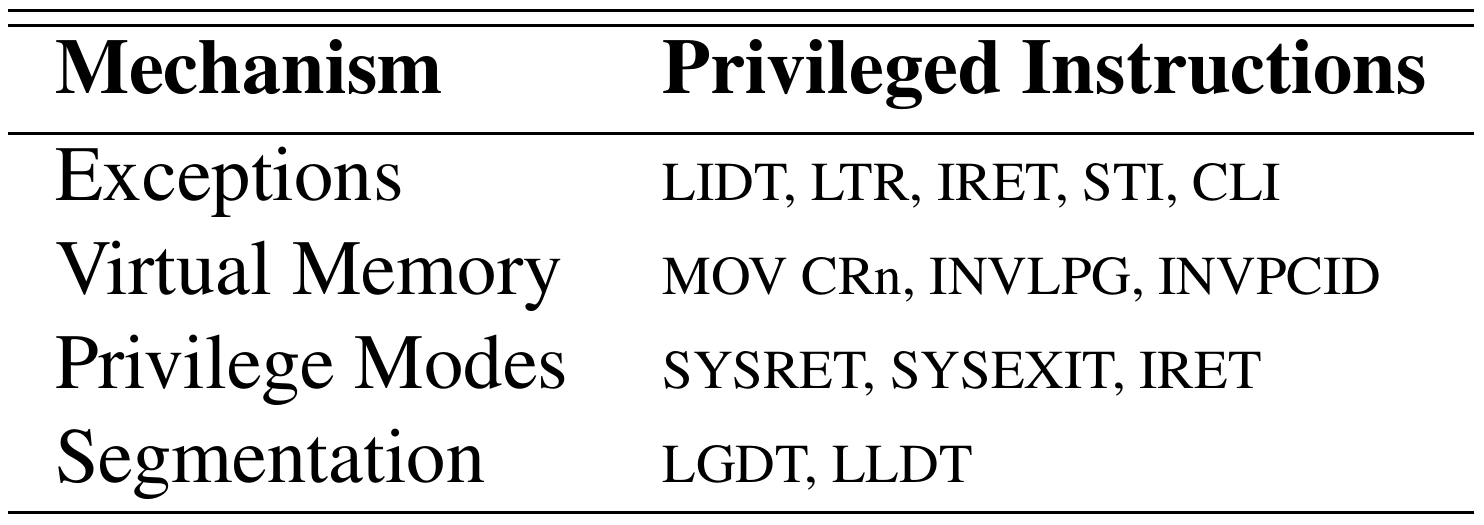
\includegraphics[width=1.\textwidth]{hw-features}
			
		\end{column}
		
		\begin{column}{.6\textwidth}
			
			
			\begin{itemize}
				\item  Two motivating use cases for
				privilege modes are privilege separation and sandboxing
				of untrusted code.
				can be performed in batches when permitted by the application. 
				\item system
				call instructions trap to the process itself, rather than to
				the kernel,
				\item can be used for system call interposition and to prevent untrusted code from directly accessing	the kernel.
				\item Compared to ptrace in Linux, we show that
				Dune can intercept a system call with 25 X less overhead
				
			\end{itemize}					
			
		\end{column}
		
		
	\end{columns}
	
	
\end{frame}



%-------------------------------------------------
\begin{frame}[plain]
	\frametitle{ Supported Hardware Features -- Privilege Modes}
	
	\centering
	
	
	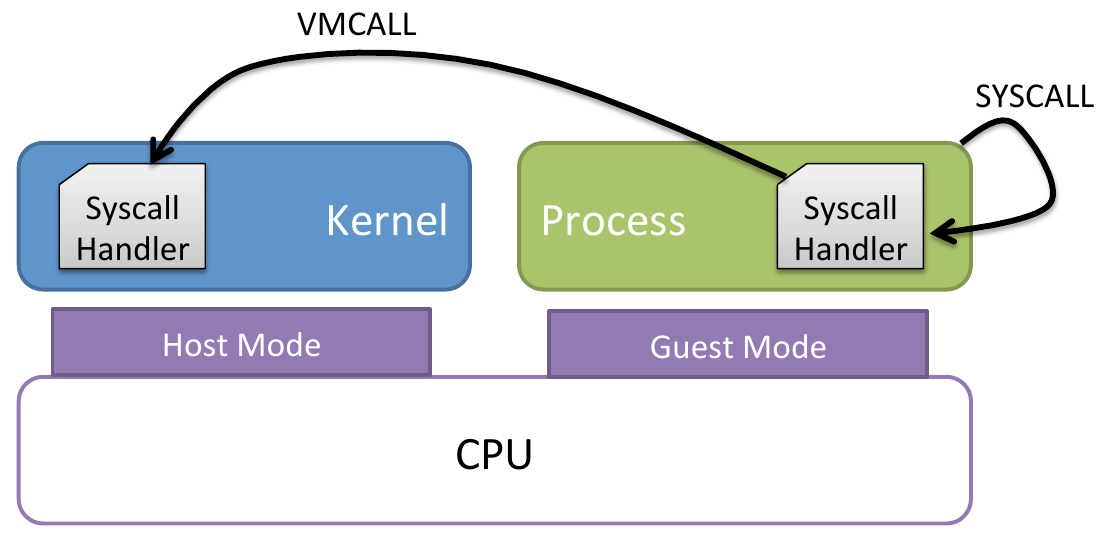
\includegraphics[width=.7\textwidth]{dune-hw-syscall}
	
	\begin{itemize}
		\item  SYSCALL	
 will	
 only	
 trap	
 back	
 into	
 the	
 process	
  
		
		\item Use	
 VMCALL	
 (i.e.	
 a	
 hypercall)	
 to	
 perform	normal	
 kernel	
 system	
 calls	
 
		
	\end{itemize}	
	
\end{frame}


%-------------------------------------------------
\begin{frame}[plain]
	\frametitle{ Supported Hardware Features -- Privilege Modes}
	
	\centering
	
	
	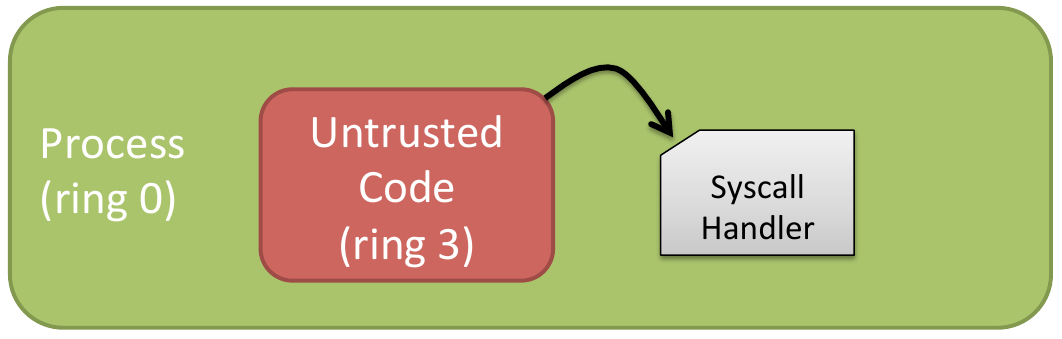
\includegraphics[width=.7\textwidth]{dune-hw-syscall-useful}
	
	\begin{itemize}
		\item  Isolate	
 untrusted	
 code	
 by	
 running	
 it	
 in	
 a	
 less	privileged	
 mode	
 (i.e.	
 ring	
 3	
 on	
 x86)	 
		
		\item Leverage	
 the	
 ‘supervisor’	
 bit	
 in	
 the	
 page	
 table	
  	to	
 protect	
 memory	
  
			
 
		
	\end{itemize}	
	
\end{frame}


%-------------------------------------------------
\begin{frame}[plain]
	\frametitle{ Implementation	 Challenges}
	
	
	
	\begin{columns}
		
		\begin{column}{.4\textwidth}
			
			
			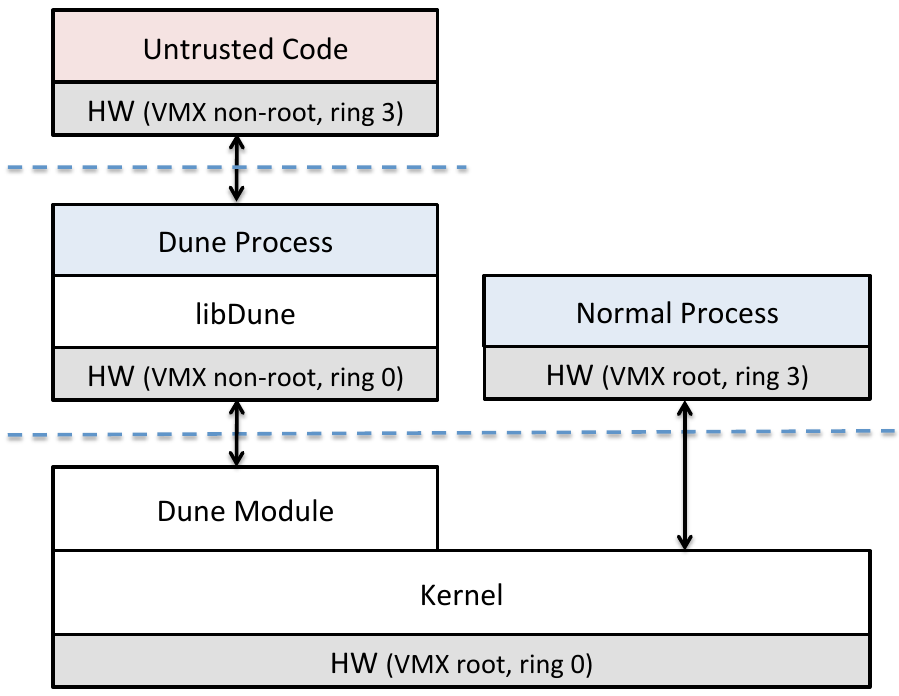
\includegraphics[width=1.\textwidth]{dune-arch}
			
		\end{column}
		
		\begin{column}{.6\textwidth}
			\begin{itemize}
			\item Reducing	VM	 exit	 and	 VM	 entry	 overhead		
			\item Pthread	 and	 fork	 were	 tricky	 to	 integrate	 with	the	 Linux	 kernel	
			\item EPT	 does	 not	 support	 enough	 address	 space	
			\item Signals	 should	 only	 be	 delivered	 to	 ring	 0, but process is in ring 3

			\end{itemize}
		\end{column}
		
		
	\end{columns}
	
	
\end{frame}


%-------------------------------------------------
\begin{frame}[plain]
	\frametitle{ Implementation	 Challenges}
	
	
	
	\begin{columns}
		
		\begin{column}{.4\textwidth}
			
			
			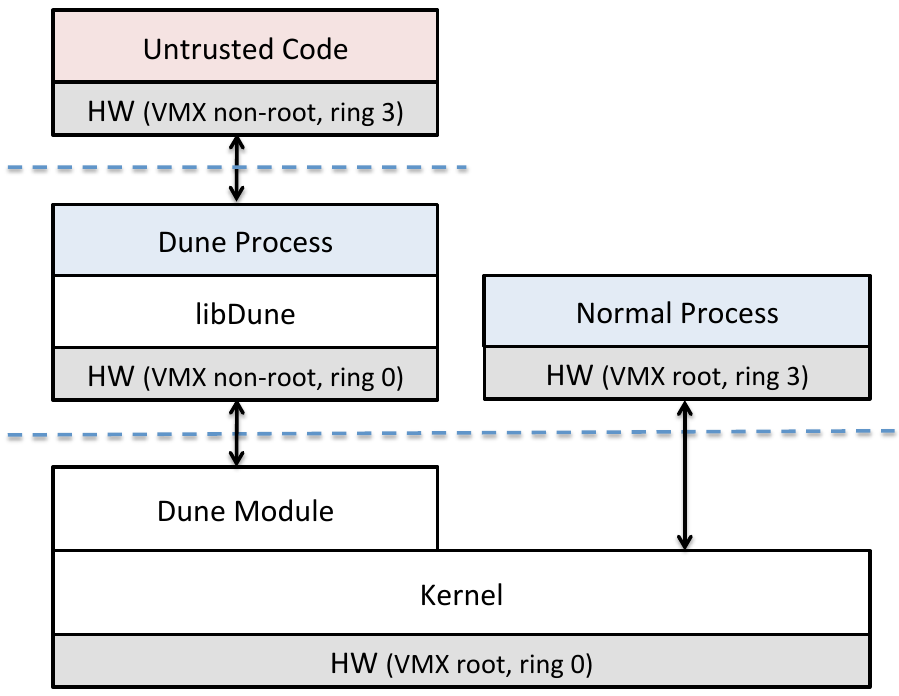
\includegraphics[width=1.\textwidth]{dune-arch}
			
		\end{column}
		
		\begin{column}{.6\textwidth}
			\begin{itemize}
				\item Reducing	VM	 exit	 and	 VM	 entry	 overhead
			\end{itemize}
		
		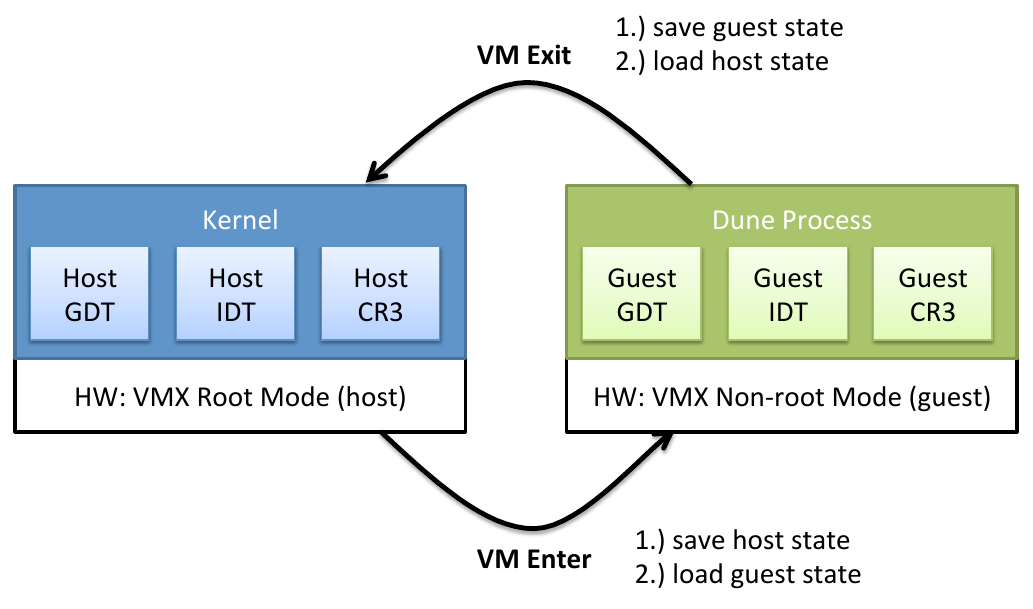
\includegraphics[width=1.\textwidth]{dune-vtx-state}
		\end{column}
		
		
	\end{columns}
	
	
\end{frame}


%-------------------------------------------------
\begin{frame}[plain]
	\frametitle{ Implementation	 Challenges}
	
	
	
	\begin{columns}
		
		\begin{column}{.4\textwidth}
			
			
			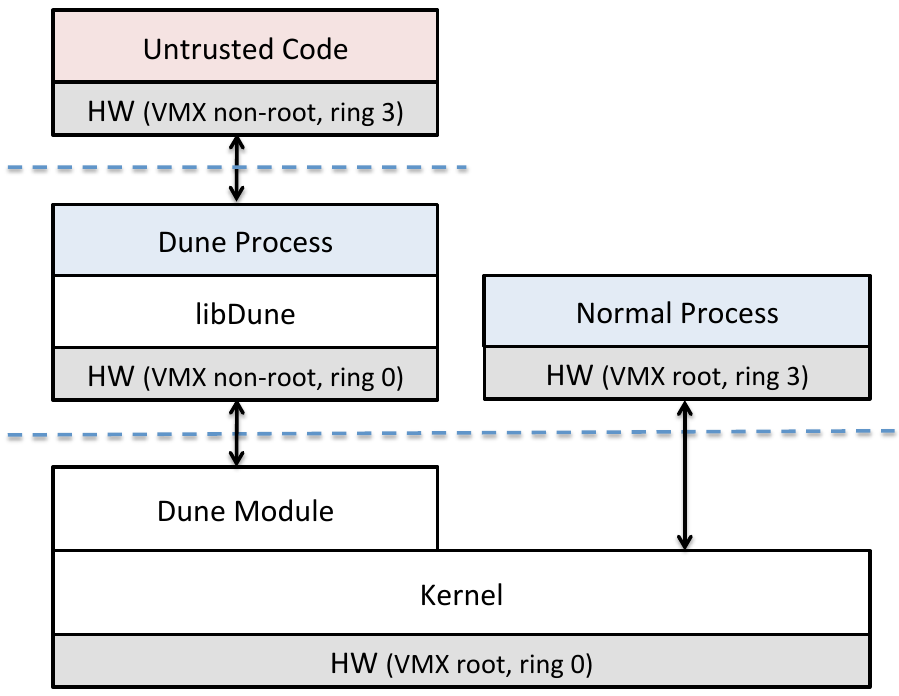
\includegraphics[width=1.\textwidth]{dune-arch}
			
		\end{column}
		
		\begin{column}{.6\textwidth}
			\begin{itemize}
				\item Application: garbage	collection
			\end{itemize}
			
			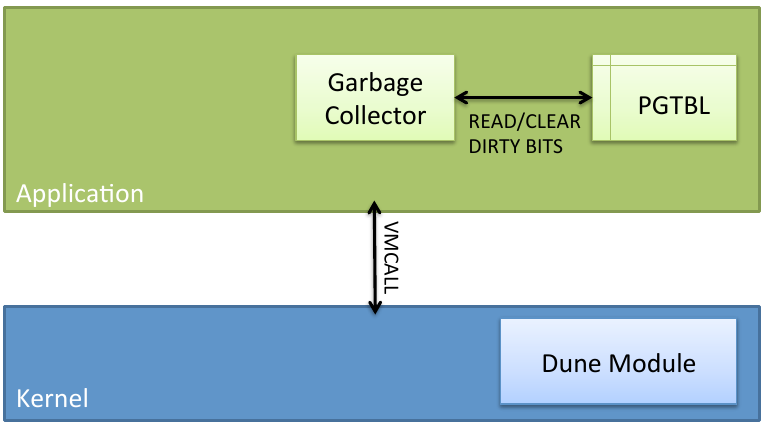
\includegraphics[width=1.\textwidth]{dune-app-garbage}
		\end{column}
		
		
	\end{columns}
	
	
\end{frame}



%-------------------------------------------------
\begin{frame}[plain]
	\frametitle{ Implementation	 Challenges}
	
	
	
	\begin{columns}
		
		\begin{column}{.4\textwidth}
			
			
			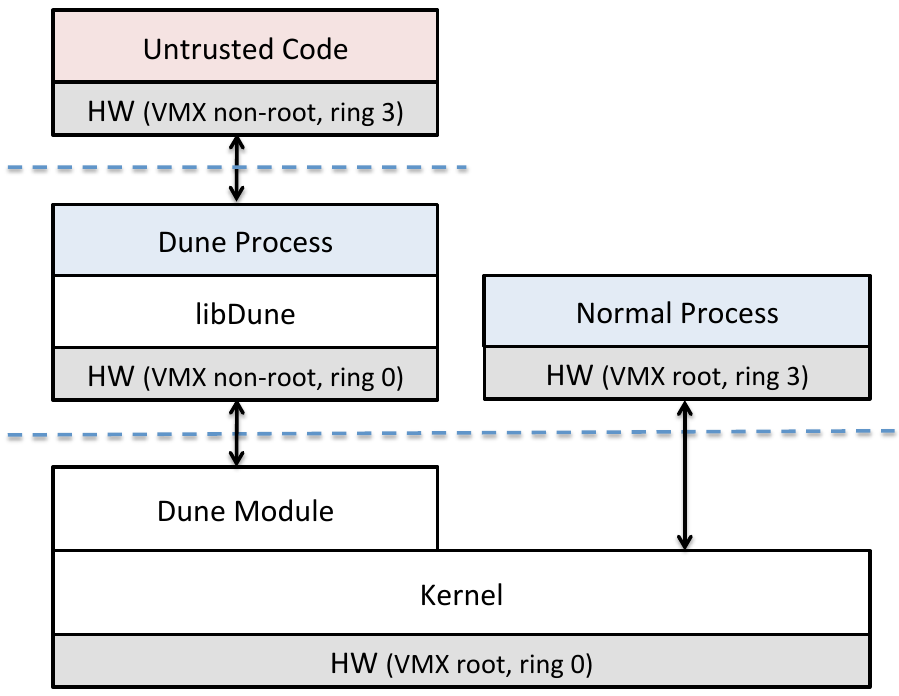
\includegraphics[width=1.\textwidth]{dune-arch}
			
		\end{column}
		
		\begin{column}{.6\textwidth}
			\begin{itemize}
				\item Application: sandbox
			\end{itemize}
			
			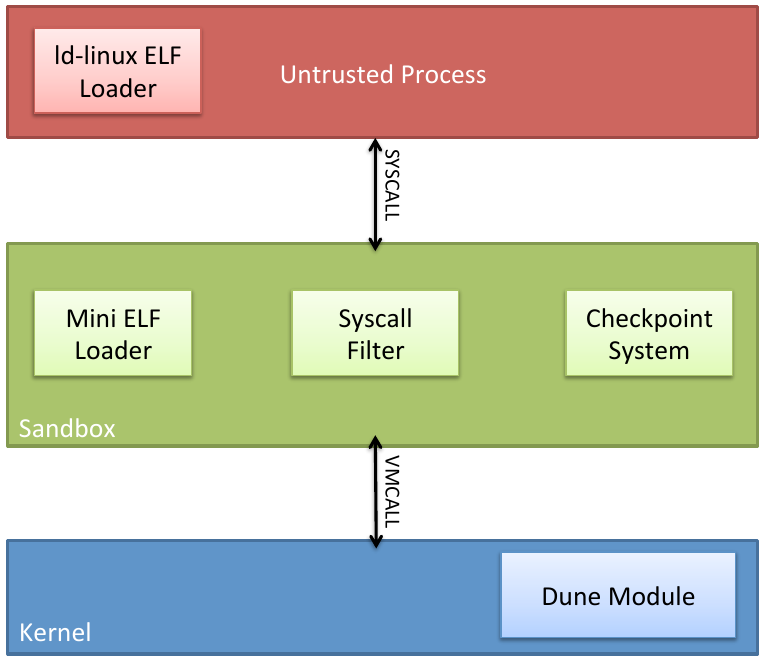
\includegraphics[width=.8\textwidth]{dune-app-sandbox}
		\end{column}
		
		
	\end{columns}
	
	
\end{frame}

%-------------------------------------------------
\begin{frame}[plain]
	\frametitle{ Performance}
	 Overhead  analysis : VMX trans, EPT trans
	 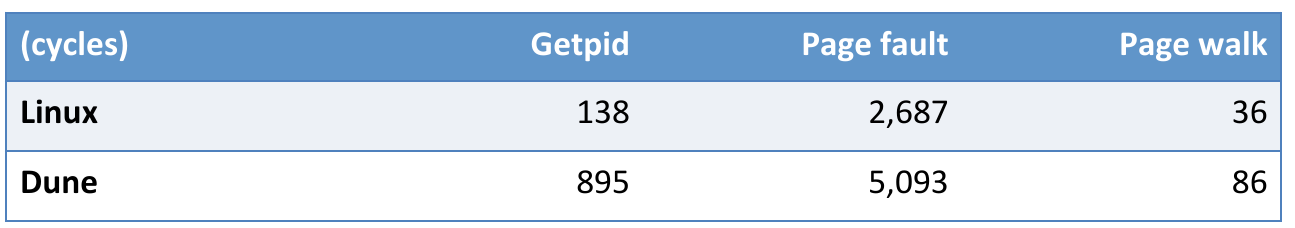
\includegraphics[width=1.\textwidth]{dune-overhead}
	
    Optimization analysis : Faster	 system	 call, Virt Mem manipulation
    
    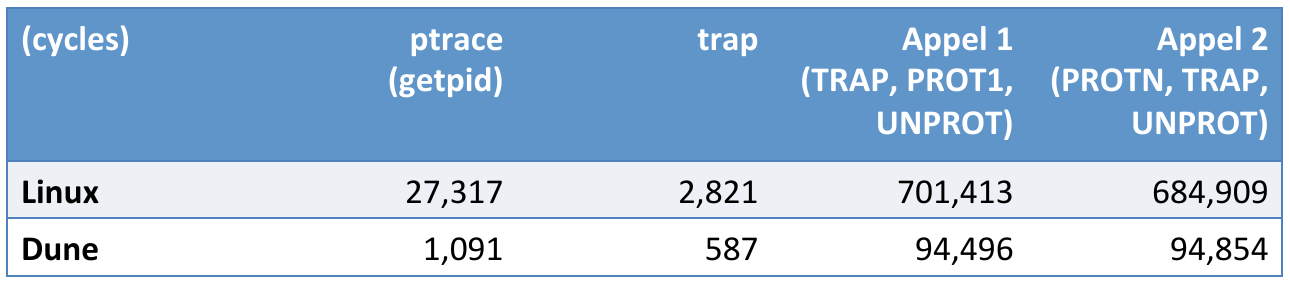
\includegraphics[width=1.\textwidth]{dune-opti}
	
\end{frame}



%-------------------------------------------------
\begin{frame}[plain]
	\frametitle{ Performance}
	Sandbox:	 SPEC2000	 performance
	
	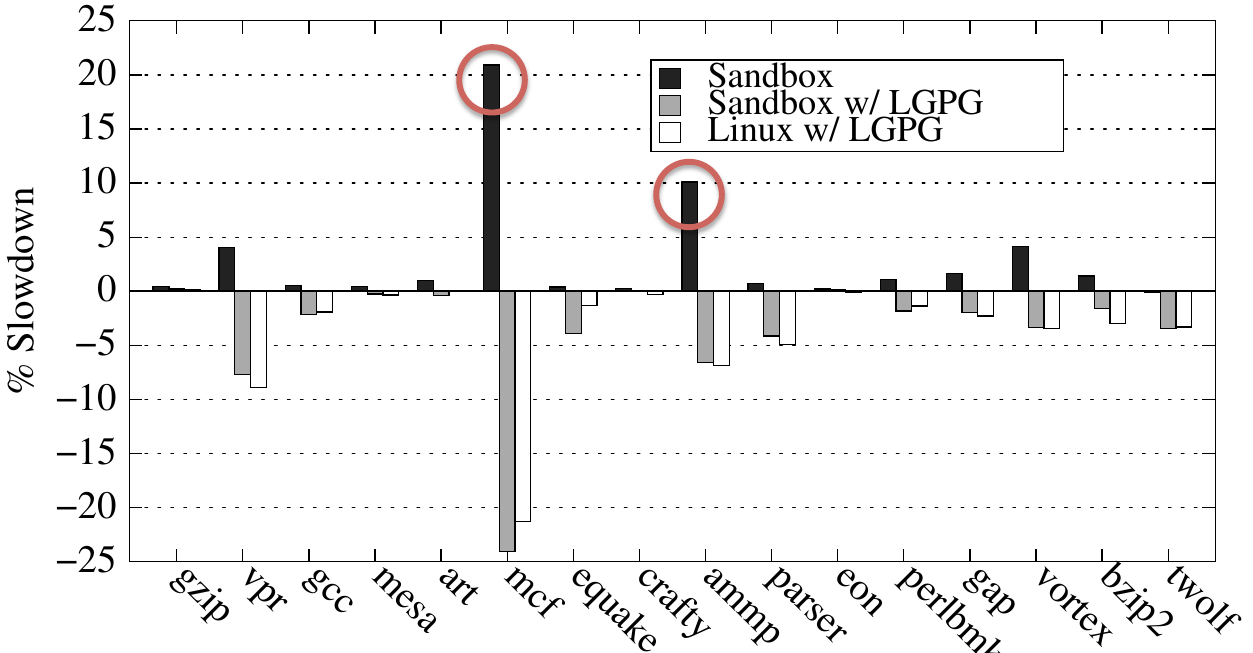
\includegraphics[width=.8\textwidth]{bench-sandbox-spec2k}
	
	 EPT overhead: use of large pages
	

	
\end{frame}



%-------------------------------------------------
\begin{frame}[plain]
	\frametitle{ Performance}
	Sandbox:	Lighttpd	
 performance	
  
	
	
	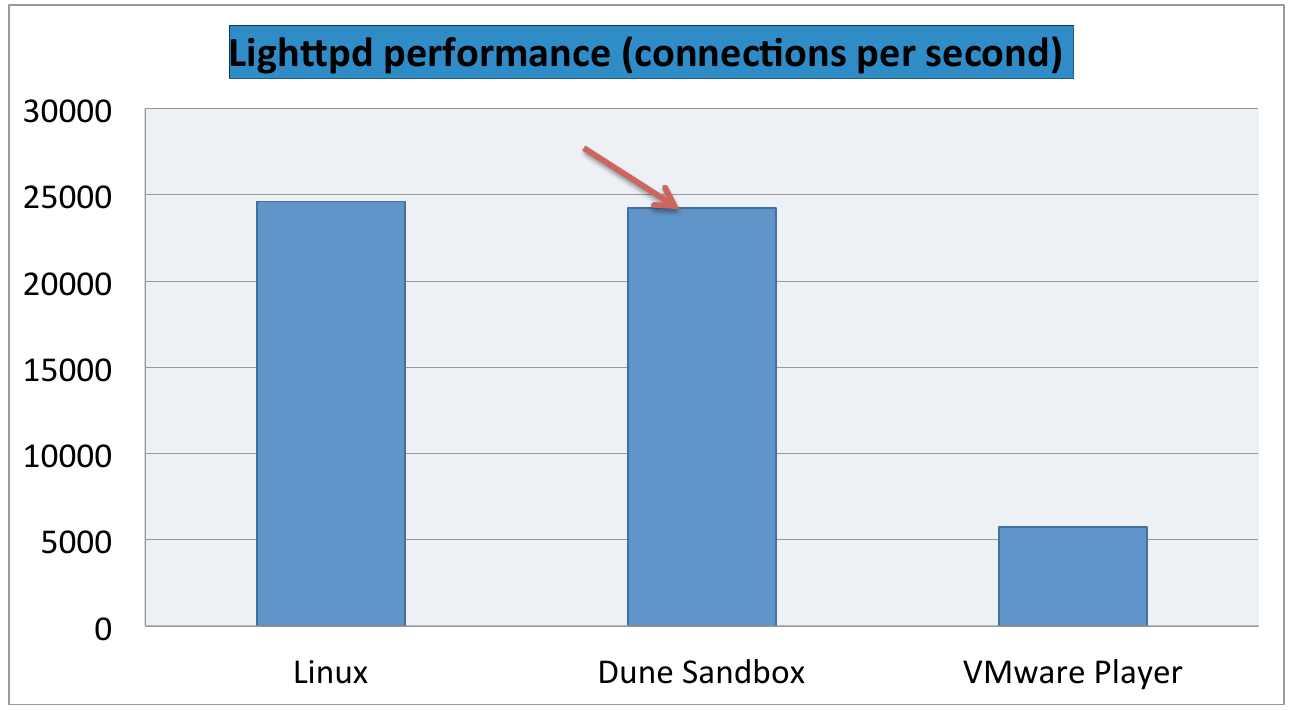
\includegraphics[width=.8\textwidth]{bench-sandbox-lighttpd}
	
	 Slight	
 reduction	
 in	
 throughput	
 (less	
 than	
 2\%)	
 due	
 to	VMCALL	
 overhead	
  
	
	
	
	
\end{frame}


%-------------------------------------------------
\begin{frame}[plain]
	\frametitle{Conclusions }
	
	
	
	\begin{columns}
		
		\begin{column}{.4\textwidth}
			
			
			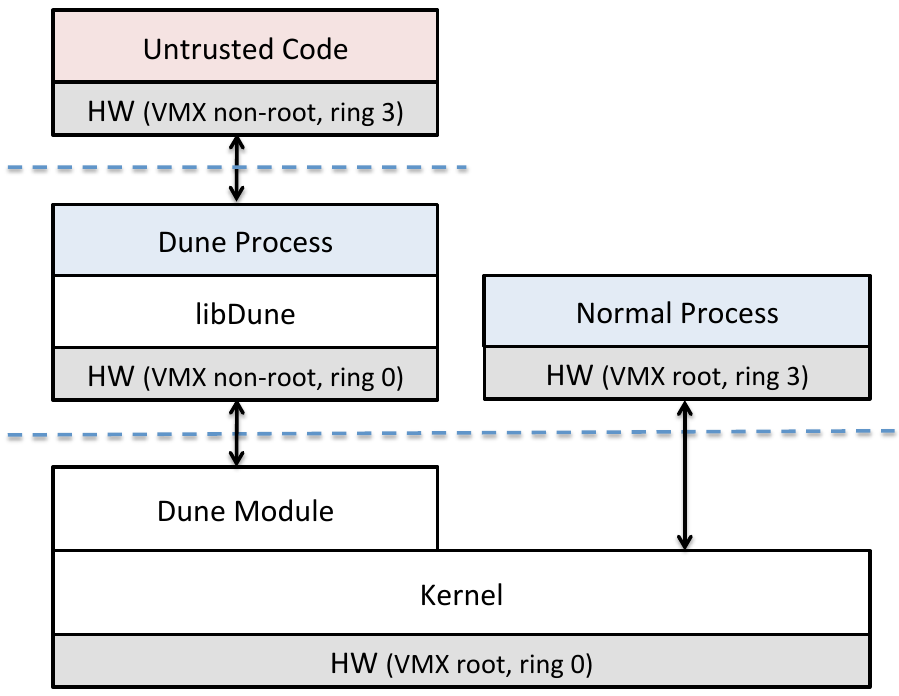
\includegraphics[width=1.\textwidth]{dune-arch}
			
		\end{column}
		
		\begin{column}{.6\textwidth}
			\begin{itemize}
				\item Applications	 can	 benefit	 from	 access	 to	 privileged	CPU	 features		
				\item Virtualization	 hardware	 allows	 us	 to	 provide	 such	access	 safely	
				\item Dune	
 creates	
 new	
 opportunities	
 to	
 build	
 and	
  
				improve	
 applications	
 without	
 kernel	
 changes	
 
				\item Dune	 has	 modest	 performance	 overhead				
			\end{itemize}
		\end{column}
		
		
	\end{columns}
	
	
\end{frame}
%-------------------------------------------------
%-------------------------------------------------
\end{document}